\documentclass{book}
\usepackage[T1]{fontenc}
\usepackage[utf8]{inputenc}
\usepackage{mystyle}




\title{CS 224W Homework 1}
\author{Yikun Chi}

\begin{document}
\maketitle

\section*{Problem 1}
\subsection*{1.1}
\begin{align*}
    & 1 \rightarrow A\\
    & 2 \rightarrow D\\
    & 3 \rightarrow H\\
    & 4 \rightarrow E\\
    & 5 \rightarrow B\\
    & 6 \rightarrow C\\
    & 7 \rightarrow G\\
    & 8 \rightarrow F\\
\end{align*}

\subsection*{1.2}
See the graph below. Let node $x$ denotes node $v_1 \in V_1$ and $v_2 \in V_2$. Let the number denotes the scalar feature value for the neighbors. So for mean and max aggregation, we have 2 for both graph. But for sum aggregation, we have 4. 

    \tikzset{every picture/.style={line width=0.75pt}} %set default line width to 0.75pt        

    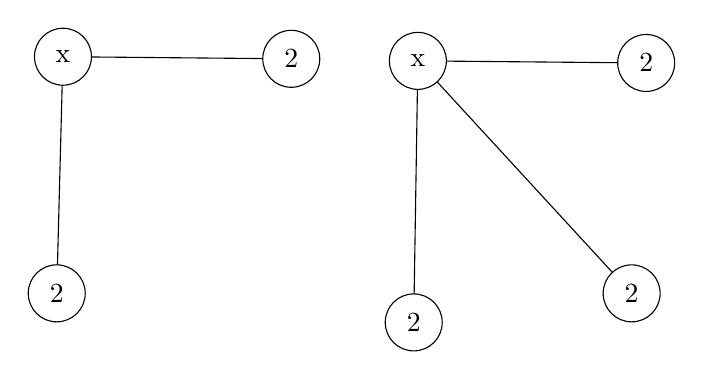
\begin{tikzpicture}[x=0.75pt,y=0.75pt,yscale=-1,xscale=1]
    %uncomment if require: \path (0,399); %set diagram left start at 0, and has height of 399
    
    
    % Text Node
    \draw    (78.38, 107.5) circle [x radius= 13.73, y radius= 13.73]   ;
    \draw (78.38,107.5) node   [align=left] {x};
    % Text Node
    \draw    (75.38, 221.5) circle [x radius= 13.73, y radius= 13.73]   ;
    \draw (75.38,221.5) node   [align=left] {2};
    % Text Node
    \draw    (188.38, 108.5) circle [x radius= 13.73, y radius= 13.73]   ;
    \draw (188.38,108.5) node   [align=left] {2};
    % Text Node
    \draw    (249.38, 109.5) circle [x radius= 13.73, y radius= 13.73]   ;
    \draw (249.38,109.5) node   [align=left] {x};
    % Text Node
    \draw    (247.38, 235.5) circle [x radius= 13.73, y radius= 13.73]   ;
    \draw (247.38,235.5) node   [align=left] {2};
    % Text Node
    \draw    (359.38, 110.5) circle [x radius= 13.73, y radius= 13.73]   ;
    \draw (359.38,110.5) node   [align=left] {2};
    % Text Node
    \draw    (352.38, 221.5) circle [x radius= 13.73, y radius= 13.73]   ;
    \draw (352.38,221.5) node   [align=left] {2};
    % Connection
    \draw    (78.01,121.22) -- (75.74,207.78) ;
    % Connection
    \draw    (92.1,107.62) -- (174.65,108.38) ;
    % Connection
    \draw    (249.16,123.23) -- (247.59,221.77) ;
    % Connection
    \draw    (263.1,109.62) -- (345.65,110.38) ;
    % Connection
    \draw    (258.67,119.61) -- (343.08,211.39) ;
    
    \end{tikzpicture}


\subsection*{1.3}
We want to proof
    \begin{align*}
        \left(\textrm{readout}\left( \{ h_v^{(K)}, \forall v\in V_1 \} \right) \neq \textrm{readout}\left( \{ h_v^{(K)}, \forall v\in V_2 \} \right) \right)
        \Longrightarrow 
        \left(WL(G_1) \neq WL(G_2) \right)
    \end{align*}
We can prove the contrapositive statement: when $G_1$ and $G_2$ isomorphic relation can not decided by WL test, then we can not determine the isomorphic relation using our readout test. \\

First we want to show that in WL test: $\{ l_v^{(K)}, \forall v\in V_1 \} = \{ l_v^{(K)}, \forall v\in V_2 \} \Longrightarrow \{ l_v^{(K-1)}, \forall v\in V_1 \} = \{ l_v^{(K-1)}, \forall v\in V_2 \}$. This is true by definition of hash function (assuming no collision). If the multiset at $K-1$ are different for $G_1$ and $G_2$, then there must exists a node $v_1$ in $G_1$ and node $v_2$ in $G_2$ such that the multiset neighbor of $v_1$ and multiset neighbor of $v_2$ at the end $K-1$ iteration are different. This implies that their hash value at K iteration will be different.  \\

Next we want to show that hashing function is more expressive than aggregate and combine function. i.e.: For a given node $u$ in $G_1$ and $x$ in $G_2$. Equal hashing of the node and its multiset neighbor hash implies equal aggregate and mean. This can also be established by the definition of hashing. We can think of it from iteration 1 when we are hashing the node features. Same hashing implies same set of node features, which implies same aggregation and combine result. \\

Combine 1 and 2 statement, we now have that at the $K$ iteration if the hashing multiset is the same, then the result of the embedding multiset also must be the same. So there will not exists a readout function that can distinguish two sets. So the embedding algorithm can not establish non-isomerism if WL test did not do so. 


\newpage 
\section*{Problem 2}
\subsection*{2.1}
Let the embedding for both $A, B, C$ to be $[2,2]^T$ and let the embedding of relations to be $[0,0]^T$. So now the simple objective is 0.
    \tikzset{every picture/.style={line width=0.75pt}} %set default line width to 0.75pt        
    
    \begin{tikzpicture}[x=0.75pt,y=0.75pt,yscale=-1,xscale=1]
    %uncomment if require: \path (0,399); %set diagram left start at 0, and has height of 399
    
    
    % Text Node
    \draw    (78.38, 107.5) circle [x radius= 14.01, y radius= 14.01]   ;
    \draw (78.38,107.5) node   [align=left] {A};
    % Text Node
    \draw    (78.38, 253.5) circle [x radius= 14.01, y radius= 14.01]   ;
    \draw (78.38,253.5) node   [align=left] {B};
    % Text Node
    \draw    (188.38, 108.5) circle [x radius= 14.3, y radius= 14.3]   ;
    \draw (188.38,108.5) node   [align=left] {C};
    % Connection
    \draw    (78.38,121.51) -- (78.38,236.49) ;
    \draw [shift={(78.38,239.49)}, rotate = 270] [fill={rgb, 255:red, 0; green, 0; blue, 0 }  ][line width=0.08]  [draw opacity=0] (8.93,-4.29) -- (0,0) -- (8.93,4.29) -- cycle    ;
    % Connection
    \draw    (92.38,107.63) -- (171.08,108.34) ;
    \draw [shift={(174.08,108.37)}, rotate = 180.52] [fill={rgb, 255:red, 0; green, 0; blue, 0 }  ][line width=0.08]  [draw opacity=0] (8.93,-4.29) -- (0,0) -- (8.93,4.29) -- cycle    ;
    
    \end{tikzpicture}


\subsection*{2.2}
Above example in 2.1 still works in this case. We can not etablish whether B and C are connected just based on embedding. So conceptually, the existence of the $\gamma$ term forces us to push the distance $d(h' + l, t')$ to be large so we can reduce the $\gamma$ impact on the error. 


\subsection*{2.3}
At high level, if we do not restrict the l2 norm value of the entity, the algorithm can let the entity embedding's value to be extremely big in relation to the relation embedding. So we could consider our object now is just $[\gamma + d(h,t) - d(h,t')]_+$ and it could get minimized without learning much on the relation embedding front. . 




\subsection*{2.4}
It cannot model symmetric relations. Let the graph just be two nodes $A$ and $B$, with relation $l$ from $A$ to $B$ and also $B$ to $A$. As an example, we can image $A$ and $B$ are person, and relation is roommate. So $A$ is roommate of $B$ implies $B$ is rommate of $A$. Let lower cause denote embedding. if $a + l = b$ then it is not possible to get $b + l = a$ unless $l$ is 0. 



\section*{Problem 3}
\subsection*{3.1}
Symmetry: \\
TransE can not model symmetry. As an example, we can image $A$ and $B$ are person, and relation is roommate. So $A$ is roommate of $B$ implies $B$ is rommate of $A$. Let lower cause denote embedding. if $a + l = b$ then it is not possible to get $b + l = a$ unless $l$ is 0. \\

Inverse: \\
TransE can model the inverse relation. If $L$ is the inverse relation of $P$, then we can just let the embedding $l$ to be the negative of $p$. We have $a + l = b \longrightarrow a = b + (-l)$. \\

Composition: \\
TransE can model composition relations. If $Z$ is the composite relation of $X$ and $Y$, then we can just let $z = x + y$ in embedding space. 

\subsection*{3.2}
Symmetry: \\
RotateE can model symmetry. Symmetry just means that $h \circ l = t$ and $t \circ l = h$. In 2D space, we can think that if the rotation is 180 degree, then rotating twice will get back to $h$, making the statement true. There can also be certain configuration of points such that after non-360 rotation the configuration are still the same.   \\


Inverse: \\
RotateE can model the inverse relation. We have a relation $h \circ l = t$ and its inverse $t \circ p = h$, If a relation is rotating by angle $l_i$, then its inverse could be $360 - l_i$. So after applying both $L$ and $P$ we get back to the self. \\



Composition: \\
RotateE can model composition relations. The composite relation is just the combined rotation of two relations. \\

\subsection*{3.4}
The RotateE can not model 1 to $N$ relationships. Given a configuration of points and a rotation, it is not possible to get two sets of configuration post rotation. So the graph could be 


\end{document}


